\documentclass[12pt,a4paper]{article}
\usepackage{algorithm, algpseudocode, amsmath, amssymb, caption, csquotes, empheq, geometry, graphicx, hyperref, listings, multirow, physics, siunitx, subcaption, upgreek}
\usepackage[section]{placeins}

\title{Computational Physics\\Problem Set}
\author{Saleh Shamloo Ahmadi\\Student Number: 98100872}
\date{September 27, 2021}

\hypersetup{colorlinks=true}

\newcommand*{\defeq}{\mathrel{\vcenter{\baselineskip0.5ex \lineskiplimit0pt
			\hbox{\scriptsize.}\hbox{\scriptsize.}}}
			=}

\newcommand{\figpath}{../fig}

\begin{document}
	\maketitle
    \section{Fractal Generation}
    Fractals are self-similar shapes, so they can be generated by repeatedly applying mappings to a set of points.
    The fractals in this problem set can all be created with linear iterated function systems (IFS).
    The transformations for these fractals can be described with affine transformations:
    \begin{gather}
        \vb{v}_{i+1, j} = T_j\vb{v}_{i, k} + \vb{c}_j\\
        \vb{v}_{i, j} = \mqty(x_{i,j} \\ y_{i,j}) \\
        T_j = \mqty(a_j & b_j \\ c_j & d_j),\quad \vb{c}_j = \mqty(e_j \\ f_j)
    \end{gather}
    There are two ways to define the mappings: relative and absolute. Also, the fractals can be generated randomly
    with the absolute mappings.
    \subsection{Relative Mapping}
    This type of mapping is suitable for use with line-based fractals (i.e. the fractal consists of a single curve).
    In this method, the transformations are applied locally on each line; The origin of the coordinate system is set
    to on end of the line and the point on the other end of the line is transformed relative to that.
    Algorithm \ref{alg:rel} is the implementation of this method.
    \begin{algorithm}
        \caption{Fractal Generation by Relative Mapping}
        \label{alg:rel}
        \begin{algorithmic}[1]
            \Function{fractal}{$x_{init}, y_{init}, T, \vb{c}, steps$}
            \Comment{$T$ and $\vb{c}$ represent the matrix and vector for every transformation}
                \State $x \gets x_{init}$
                \State $y \gets y_{init}$
                \For{$step \gets 1,steps$}
                    \State $i \gets 1$
                    \While{$i < N(x)$}
                    \Comment{N(x) is the number of x coordinates (which is the same as the number of points)}
                        \State $\mqty(x_{rel} \\ y_{rel}) \gets \mqty(x_{i+1} - x_i \\ y_{i+1} - y_i)$
                        \ForAll{$T_j$ and $\vb{c}_j$}
                            \State $\mqty(x_{new} \\ y_{new}) \gets T_j\mqty(x_{rel} \\ y_{rel}) + \vb{c}$
                            \State insert $x_{new}$ into $x$ at index $i$
                            \State insert $y_{new}$ into $y$ at index $i$
                            \State $i \gets i+1$
                        \EndFor
                    \EndWhile
                \EndFor
                \State \textbf{return} $x$ and $y$
            \EndFunction
        \end{algorithmic}
    \end{algorithm}
    \subsection{Absolute Mapping}
    This type of mapping is suitable for non-line-based fractals (the fractal isn't only a single curve).
    In this method, the same transformations are applied to every point in each step to generate new points.
    The origin of the coordinate system is always set at the first point of the fractal. By repeatedly applying
    the transformations to the fractal in each step, the self-similar shape is created.
    Algorithm \ref{alg:abs} is the implementation of this method.
    \begin{algorithm}
        \caption{Fractal Generation by Absolute Mapping}
        \label{alg:abs}
        \begin{algorithmic}[1]
            \Function{fractal}{$x_{init}, y_{init}, T, \vb{c}, steps$}
            \Comment{$T$ and $\vb{c}$ represent the matrix and vector for every transformation}
                \State $x \gets x_{init}$
                \State $y \gets y_{init}$
                \For{$step \gets 1,steps$}
                    \State define the $x_{new}$ empty array
                    \State define the $y_{new}$ empty array
                    \ForAll{$x_i \in x$ and $y_i \in y$}
                        \ForAll{$T_j$ and $\vb{c}_j$}
                            \State $\mqty(x_{gen} \\ y_{gen}) \gets T_j\mqty(x_{rel} \\ y_{rel}) + \vb{c}$
                            \State append $x_{gen}$ to $x_{new}$
                            \State append $y_{gen}$ to $y_{new}$
                        \EndFor
                    \EndFor
                    \State $x \gets x_{new}$
                    \State $y \gets y_{new}$
                \EndFor
                \State \textbf{return} $x$ and $y$
            \EndFunction
        \end{algorithmic}
    \end{algorithm}
    \subsection{Random Fractals}
    Some fractals can be generated by repeatedly applying random transformations from the fractal. If this is done with enough
    sample points, and enough steps so that the smalles unit of the shape is smaller than a pixel of the display, the fractal
    will be perfect. Algorithm \ref{alg:rand} is the implementation of this method.
    \begin{algorithm}
        \caption{Fractal Generation by Absolute Mapping}
        \label{alg:rand}
        \begin{algorithmic}[1]
            \Function{fractal}{$range_x, range_y, T, \vb{c}, steps, samples$}
            \Comment{$T$ and $\vb{c}$ represent the matrix and vector for every transformation}
                \State generate random $x$ values in $range_x$ ($N(x)=samples$)
                \State generate random $y$ values in $range_y$ ($N(y)=samples$)
                \ForAll{$x_i \in x$ and $y_i \in y$}
                    \For{$step \gets 1,steps$}
                        \State choose random $T_j$ and $\vb{c}_j$
                        \State $\mqty(x_i \\ y_i)\gets T_j\mqty(x_i \\ y_i) + \vb{c}_j$
                    \EndFor
                \EndFor
                \State \textbf{return} $x$ and $y$
            \EndFunction
        \end{algorithmic}
    \end{algorithm}
    \subsection{Representation of the fractals}
    The fractals are defined by functions $\{f_1, f_2, \dots, f_n\}$. Each of the functions are
    \begin{equation}
        f_i(\vb{v}) = T_i\vb{v} + \vb{c}_i,
    \end{equation}
    where
    \begin{gather}
        T = \mqty(a & b \\ c & d),\quad \vb{c} = \mqty(e \\ f).
    \end{gather}
    So we can represent each fractal by defining the values $a$, $b$, $c$, $d$, $e$.
    \section{Koch Snowflake}
    \begin{table}
        \centering
        \begin{tabular}{|c|c|c|c|c|c|c|}
            \hline
            transformation & $a$ & $b$ & $c$ & $d$ & $e$ & $f$ \\
            \hline
            $f_1$ & $\flatfrac{1}{3}$ & 0 & 0 & $\flatfrac{1}{3}$ & 0 & 0 \\
            \hline
            $f_2$ & $\flatfrac{1}{6}$ & $-\flatfrac{\sqrt{3}}{6}$ & $\flatfrac{\sqrt{3}}{6}$ & $\flatfrac{1}{6}$ & $\flatfrac{1}{3}$ & 0 \\
            \hline
            $f_3$ & $\flatfrac{1}{6}$ & $-\flatfrac{\sqrt{3}}{6}$ & $\flatfrac{\sqrt{3}}{6}$ & $\flatfrac{1}{6}$ & $\flatfrac{1}{2}$ & $\flatfrac{\sqrt{3}}{6}$ \\
            \hline
            $f_4$ & $\flatfrac{1}{3}$ & 0 & 0 & $\flatfrac{1}{3}$ & $\flatfrac{2}{3}$ & 0 \\
            \hline
        \end{tabular}
    \end{table}
    \begin{figure}
        \centering
        \makebox[\linewidth][c]{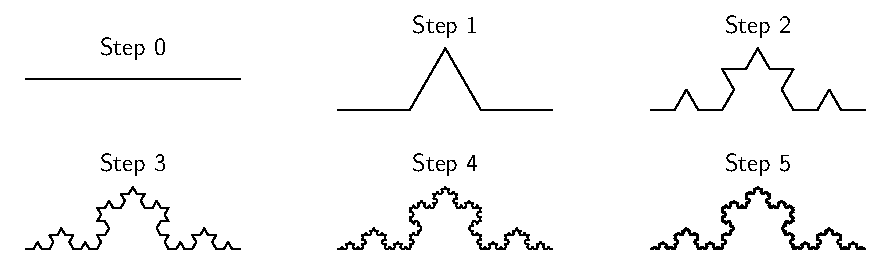
\includegraphics{\figpath/koch}}
        \makebox[\linewidth][c]{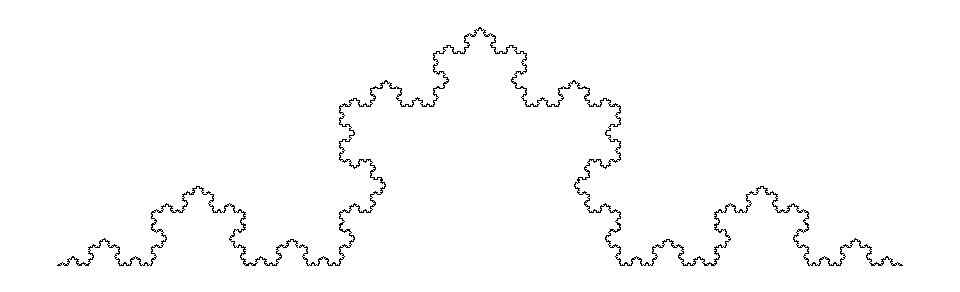
\includegraphics{\figpath/koch-large}}
        \makebox[\linewidth][c]{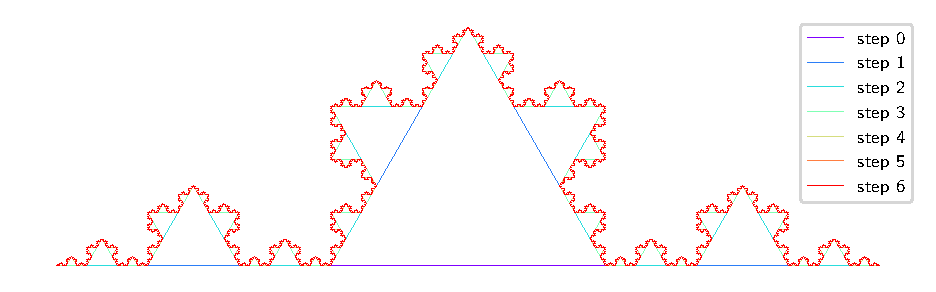
\includegraphics{\figpath/koch-color.pdf}}
        \caption{Koch Curve}
    \end{figure}
    \begin{figure}
        \centering
        \makebox[\linewidth][c]{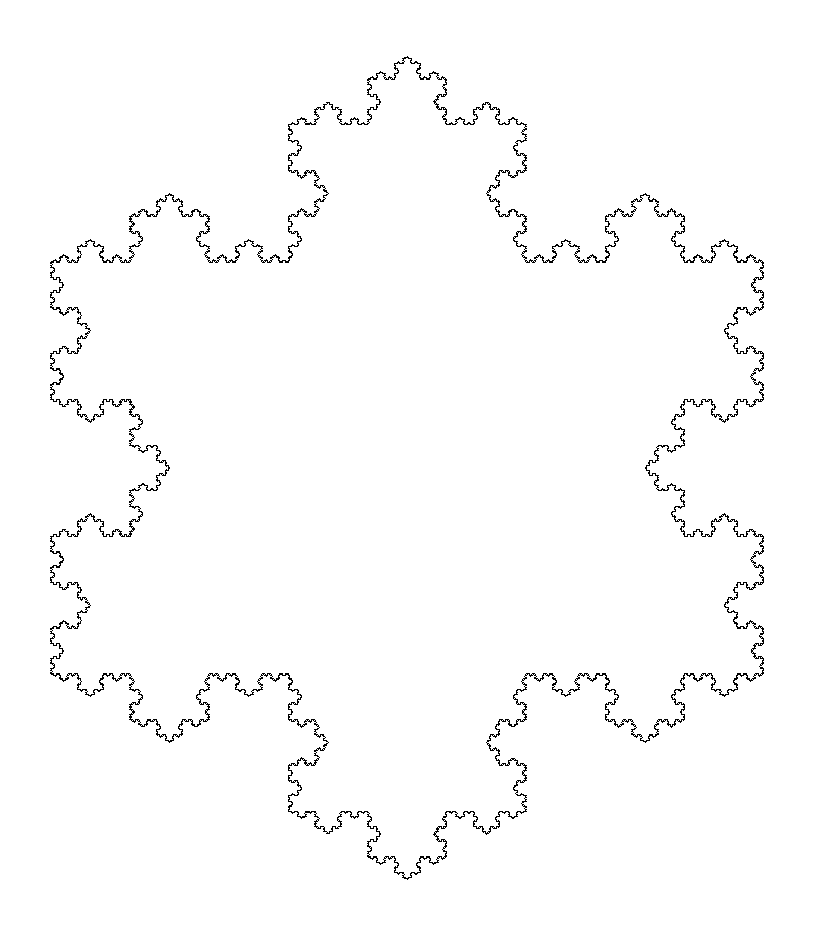
\includegraphics{\figpath/koch-tri}}
        \caption{Koch Snowflake}
    \end{figure}
    \begin{figure}
        \centering
        \makebox[\linewidth][c]{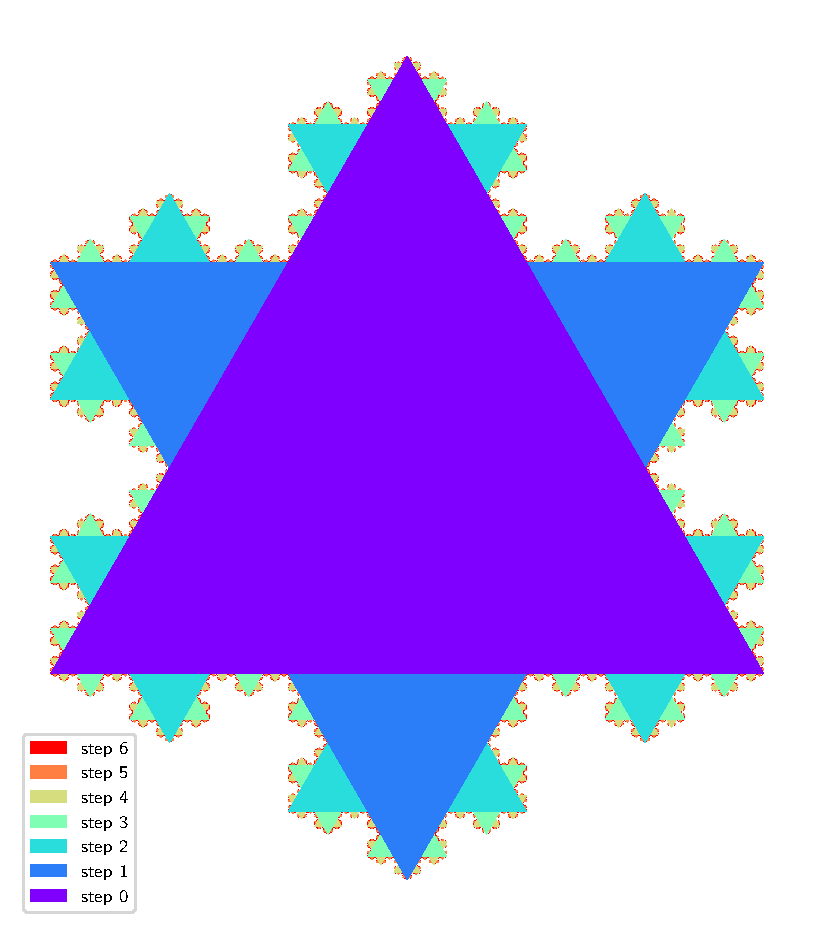
\includegraphics{\figpath/koch-tri-color}}
        \caption{Colored Koch Snowflake}
    \end{figure}
    \section{Heighway Dragon}
    \begin{table}
        \centering
        \begin{tabular}{|c|c|c|c|c|c|c|}
            \hline
            transformation & $a$ & $b$ & $c$ & $d$ & $e$ & $f$ \\
            \hline
            $f_1$ & $\flatfrac{1}{2}$ & $\flatfrac{1}{2}$ & $-\flatfrac{1}{2}$ & $\flatfrac{1}{2}$ & 0 & 0 \\
            \hline
            $f_2$ & $-\flatfrac{1}{2}$ & $\flatfrac{1}{2}$ & $-\flatfrac{1}{2}$ & $-\flatfrac{1}{2}$ & $\flatfrac{1}{2}$ & $-\flatfrac{1}{2}$ \\
            \hline
        \end{tabular}
    \end{table}
    \begin{figure}
        \centering
        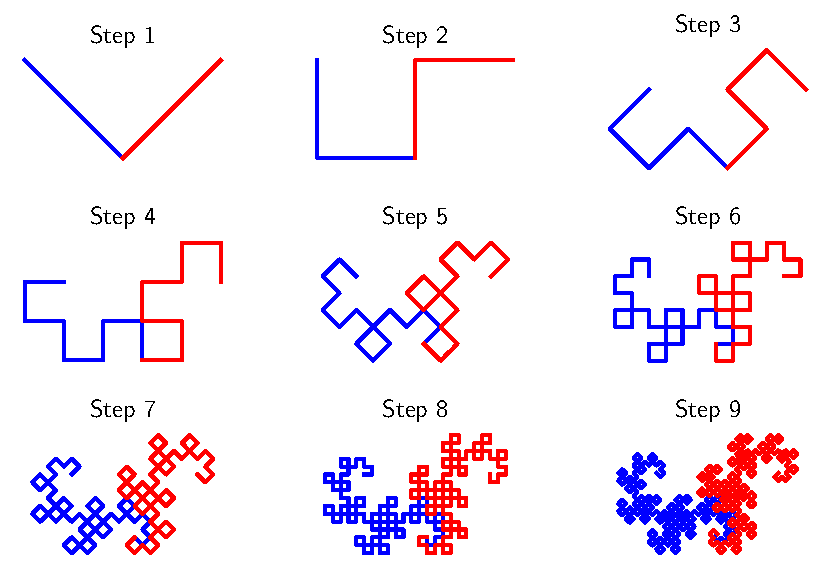
\includegraphics[width=\linewidth]{\figpath/heighway}
    \end{figure}
    \begin{figure}
        \centering
        \makebox[\linewidth][c]{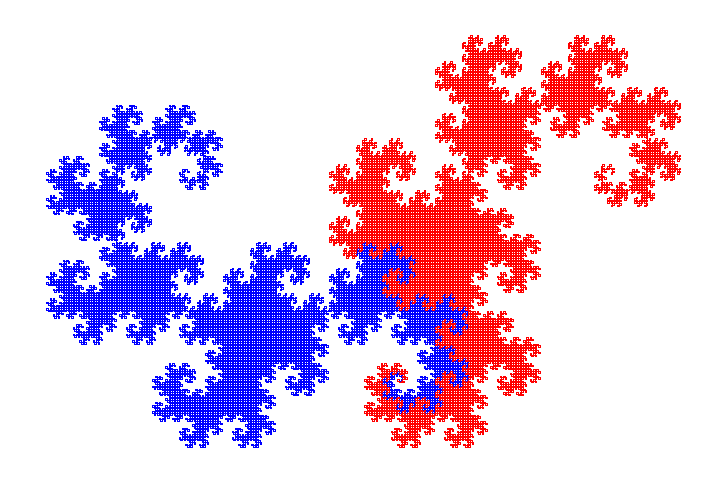
\includegraphics{\figpath/heighway-large}}
    \end{figure}
    \section{Sierpiński Triangle}
    \begin{figure}[htb!]
        \centering
        \makebox[\linewidth][c]{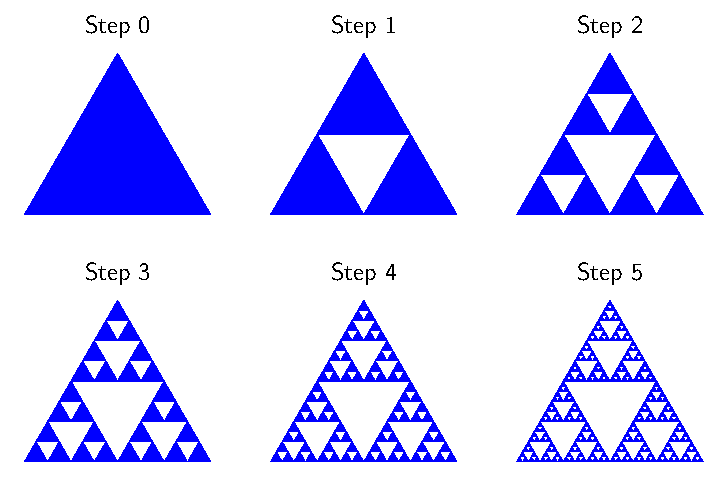
\includegraphics{\figpath/sierpinski}}
    \end{figure}
    \begin{table}
        \centering
        \begin{tabular}{|c|c|c|c|c|c|c|}
            \hline
            transformation & $a$ & $b$ & $c$ & $d$ & $e$ & $f$ \\
            \hline
            $f_1$ & $\flatfrac{1}{2}$ & 0 & 0 & $\flatfrac{1}{2}$ & 0 & 0 \\
            \hline
            $f_2$ & $\flatfrac{1}{2}$ & 0 & 0 & $\flatfrac{1}{2}$ & $\flatfrac{1}{4}$ & $\flatfrac{\sqrt{3}}{4}$ \\
            \hline
            $f_3$ & $\flatfrac{1}{2}$ & 0 & 0 & $\flatfrac{1}{2}$ & $\flatfrac{1}{2}$ & 0 \\
            \hline
        \end{tabular}
    \end{table}
    \begin{figure}
        \centering
        \centering
        \makebox[\linewidth][c]{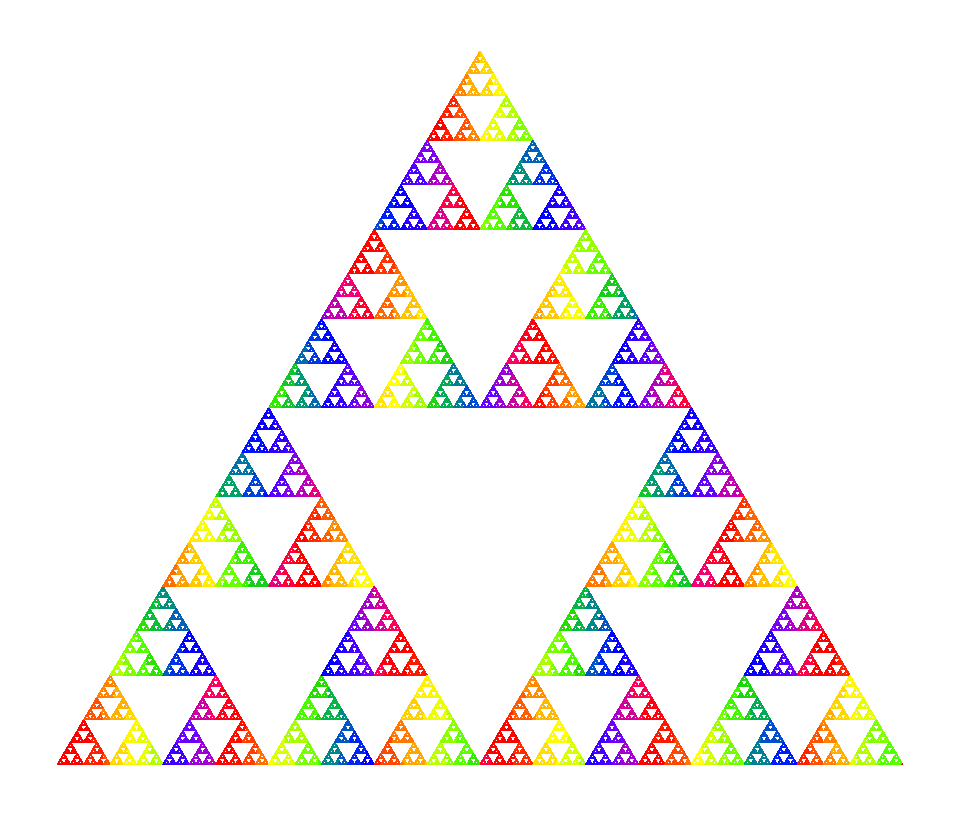
\includegraphics{\figpath/sierpinski-large}}
        \caption{Step 10 Sierpiński triangle}
    \end{figure}
    \newgeometry{top=0.4in}
    \thispagestyle{empty}
    \begin{figure}
        \centering
        \begin{subfigure}{\linewidth}
            \centering
            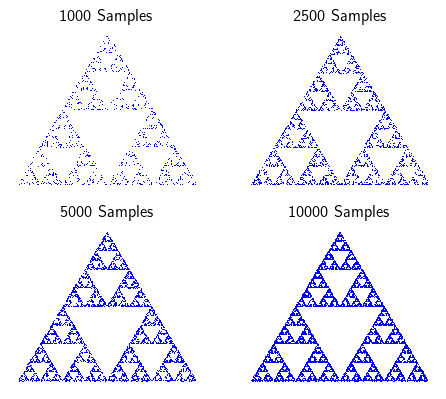
\includegraphics[width=\linewidth]{\figpath/sierpinski-random}
        \end{subfigure}
        \begin{subfigure}{\linewidth}
            \centering
            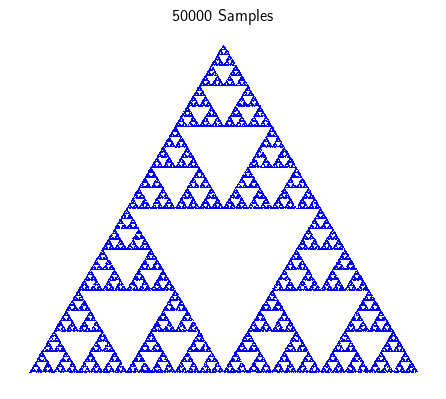
\includegraphics[width=\linewidth]{\figpath/sierpinski-random-large}
        \end{subfigure}
        \caption{Randomly Generating the Sierpiński Triangle}
    \end{figure}
    \FloatBarrier
    \restoregeometry
    \subsection{The Sierpiński Triangle Inside Pascal's Triangle}
    \newgeometry{left=0in,right=0in}
    \begin{figure}
        \centering
        \begin{subfigure}{0.45\linewidth}
            \centering
            \makebox[0.45\linewidth][c]{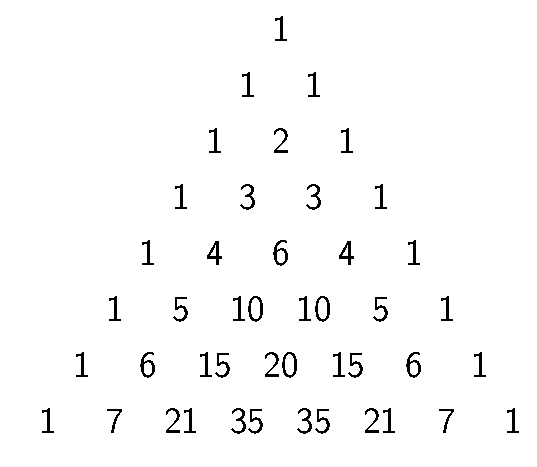
\includegraphics{\figpath/pascal-triangle}}
            \caption{Pascal's Triangle}
        \end{subfigure}
        \begin{subfigure}{0.45\linewidth}
            \centering
            \makebox[0.45\linewidth][c]{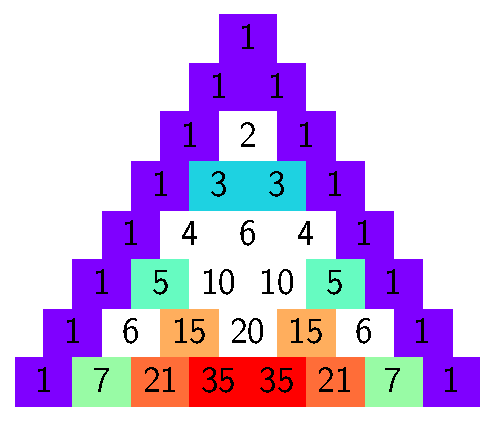
\includegraphics{\figpath/pascal-triangle-fractal}}
            \caption{Connecting the odd numbers generates the Sierpiński triangle}
        \end{subfigure}
        \begin{subfigure}{0.45\linewidth}
            \centering
            \makebox[0.45\linewidth][c]{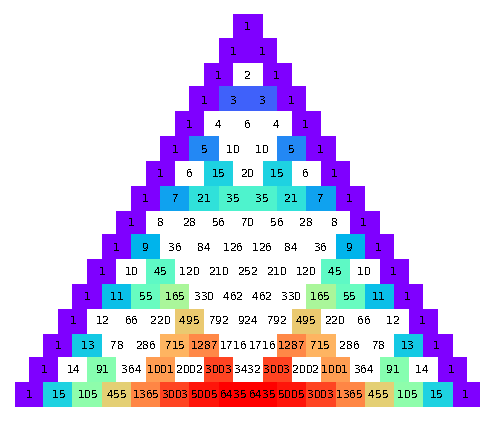
\includegraphics{\figpath/pascal-fractal}}
            \caption{The Sierpiński triangle inside a larger Pascal's triangle}
        \end{subfigure}
        \begin{subfigure}{0.45\linewidth}
            \centering
            \makebox[0.45\linewidth][c]{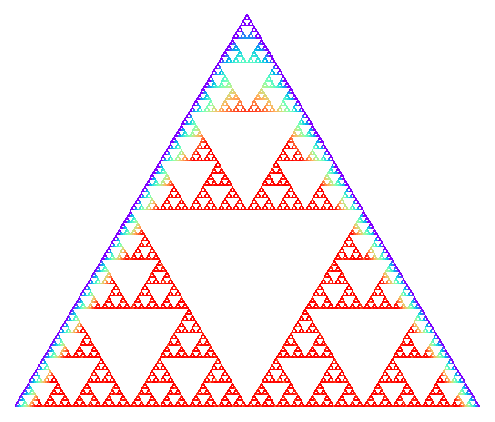
\includegraphics{\figpath/pascal-fractal-large}}
            \caption{Painted on Pascal's triangle of size 256}
        \end{subfigure}
    \end{figure}
    \FloatBarrier
    \restoregeometry
    \section{Barnsley Fern}
    To create this fractal, we need to apply random functions with different probabilities.
    \begin{table}
        \centering
        \begin{tabular}{|c|c|c|c|c|c|c|c|}
            \hline
            transformation & $a$ & $b$ & $c$ & $d$ & $e$ & $f$ & probability \\
            \hline
            $f_1$ & 0 & 0 & 0 & 0.16 & 0 & 0 & 1\% \\
            \hline
            $f_2$ & 0.85 & 0.04 & -0.04 & 0.85 & 0 & 1.6 & 85\% \\
            \hline
            $f_3$ & 0.20 & -0.26 & 0.23 & 0.22 & 0 & 1.6 & 7\% \\
            \hline
            $f_4$ & -0.15 & 0.28 & -0.26 & 0.24 & 0 & 0.44 & 7\% \\
            \hline
        \end{tabular}
    \end{table}
    \thispagestyle{empty}
    \begin{figure}
        \centering
        \makebox[\linewidth][c]{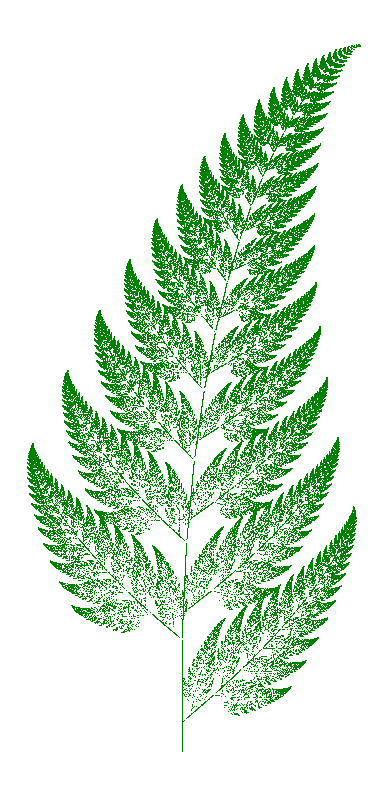
\includegraphics{\figpath/barnsley-fern}}
        \caption{Barnsley fern with 200000 random samples and 25 transformation steps}
    \end{figure}
\end{document}
